\section{Kinematics and Gait Planning}

\subsection{Inverse Kinematics}

To mandate the endpoint position $(x, y, z)$ of each limb relative
to the geometric origin of the base frame, a nonlinear inverse
kinematics (IK) model \cite{craig2005introduction} derives the required articular angles
$(\theta_1, \theta_2, \theta_3)$ for the hip, thigh, and calf
joints. The physical topology structuring the Cartesian workspace
includes a platform length of $L=250$ mm, a platform width of
$W=193$ mm, and individual linkage spans $l_1=45$ mm, $l_2=107$ mm,
and $l_3=116$ mm.

The mathematical solution avoids geometric singularities by
enforcing strictly restricted bounding limits calculated dynamically
during system initialization. Fig.~\ref{fig:kinematic_model}
illustrates the reference frame assignments at each joint
origin, with RGB axes denoting the local coordinate systems
used for forward and inverse kinematic resolution.

\begin{figure}[htbp]
    \centering
    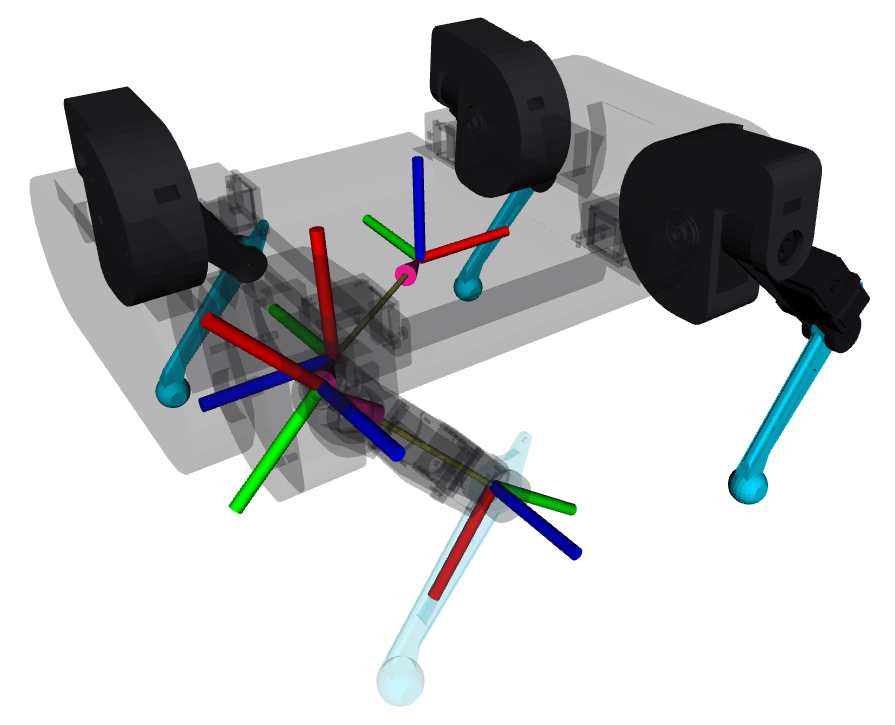
\includegraphics[width=0.38\textwidth]{figures/model_referenceframe.png}
    \caption{Simulation model with reference frames visualized at
    each joint. Each joint origin displays RGB axis indicators
    (red=$x$, green=$y$, blue=$z$) used for geometric IK
    resolution across the three DOF limb topology.}
    \label{fig:kinematic_model}
\end{figure}

\subsection{Quintic Trajectory Formulation}

Minimizing ground impact velocity is mathematically imperative;
violent mechanical shocks corrupt inertial sensor baselines and
induce structural fatigue \cite{kajita2003biped}. Therefore, foot
trajectories are shaped using the normalized quintic interpolation
function:

\begin{equation}
    s(\tau) = 10\tau^3 - 15\tau^4 + 6\tau^5
    \label{eq:quintic_s}
\end{equation}

\noindent where $\tau = t / T \in [0, 1]$ and $s \in [0, 1]$.
This function enforces the critical boundary conditions:

\begin{align}
    s(0) &= 0, \quad s(1) = 1 \nonumber\\
    \dot{s}(0) &= \dot{s}(1) = 0 \\
    \ddot{s}(0) &= \ddot{s}(1) = 0 \nonumber
\end{align}

The resulting velocity and acceleration profiles are obtained by
differentiation:

\begin{equation}
    \dot{s}(\tau) = \frac{1}{T}(30\tau^2 - 60\tau^3 + 30\tau^4)
\end{equation}

\begin{equation}
    \ddot{s}(\tau) = \frac{1}{T^2}(60\tau - 180\tau^2 + 120\tau^3)
\end{equation}

Fig.~\ref{fig:trajectory_combined}a visualizes the position,
velocity, and acceleration profiles, confirming the enforced
zero derivative boundary conditions.

For the swing phase of duration $T_{swing}=70$ frames, the foot
transitions from liftoff coordinate $\mathbf{A}$ to touchdown
coordinate $\mathbf{D}$ along a D shaped parabolic arc with
configurable lift height $h_{lift}=40$ mm:

\begin{align}
    \mathbf{p}_{swing}(\tau) &= \mathbf{A}
    + s(\tau)(\mathbf{D} - \mathbf{A}) \\
    z(\tau) &= z_{ground}
    + 4 h_{lift} \cdot s(\tau)(1 - s(\tau))
\end{align}

The resulting D shaped foot path is illustrated in
Fig.~\ref{fig:gait_3d}, showing the swing arc and ground
retrace phases with annotated liftoff and touchdown boundaries.

\begin{figure}[htbp]
    \centering
    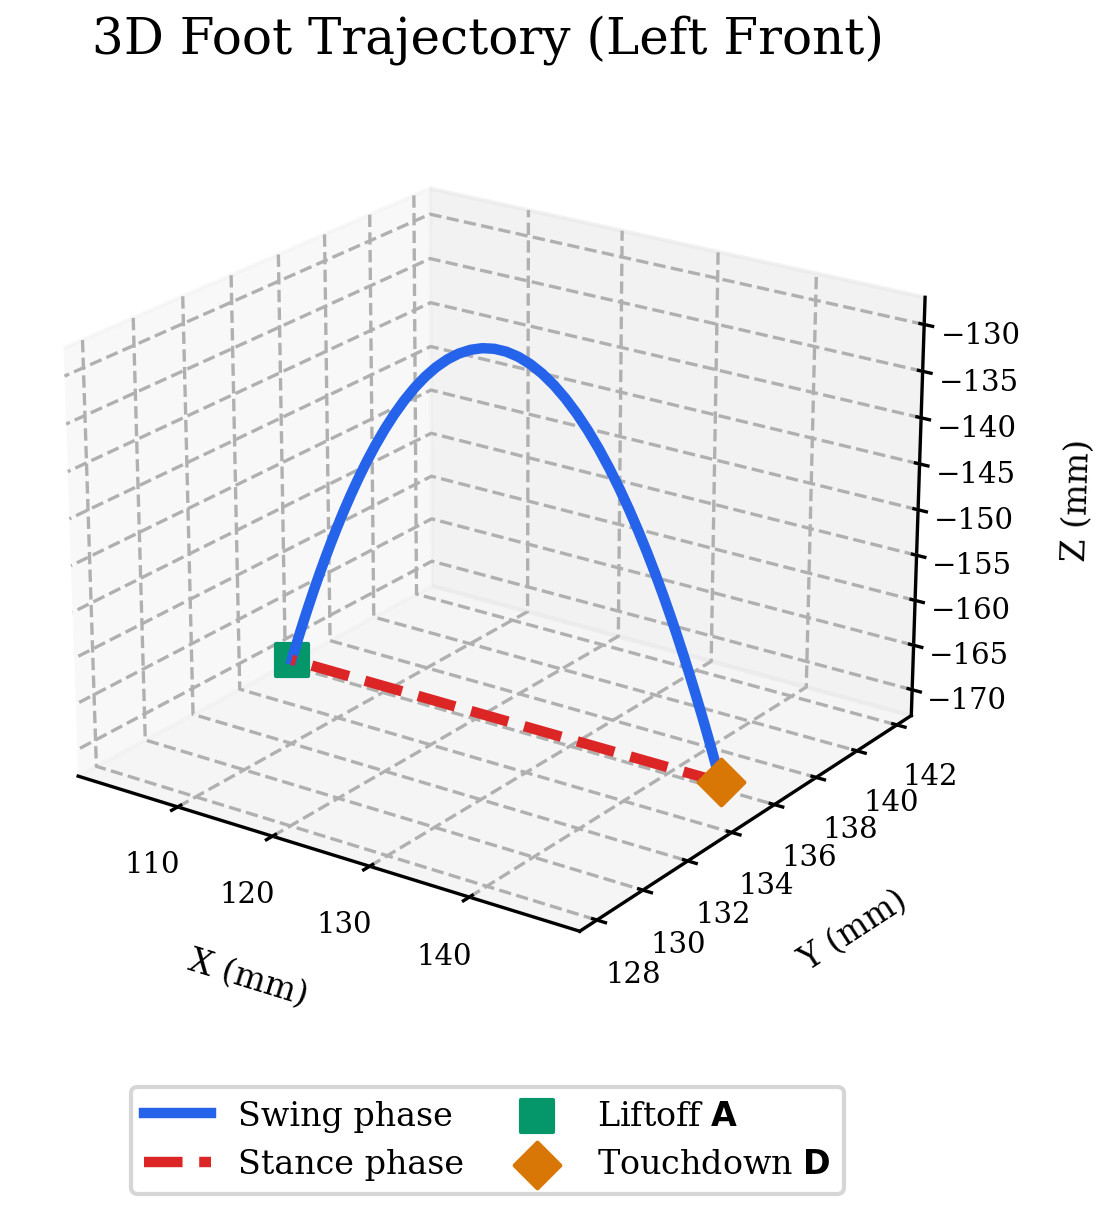
\includegraphics[width=0.65\columnwidth]{figures/gait_trajectory_3d.png}
    \caption{3D foot trajectory for the left front limb. The swing
    phase (blue) traces a quintic parabolic arc from liftoff
    $\mathbf{A}$ to touchdown $\mathbf{D}$, while the stance
    phase (red dashed) retraces along the ground plane at
    $z=-170$ mm. Stride length $L_{stride}=45$ mm,
    lift height $h_{lift}=40$ mm.}
    \label{fig:gait_3d}
\end{figure}

During the stance phase of duration $T_{stance}=200$ frames, the
foot retraces along the ground plane using the same quintic
interpolation to ensure smooth velocity profiles in the reverse
direction. The stride length is set at $L_{stride}=45$ mm, centered
about each leg's neutral $x_{center}$ position.

Overlapping gaits involving multiple limbs are generated by applying
phase shift offsets $\phi_i$ to the trajectory index for each limb.
For a standard trot, diagonal pairs share identical phase offsets
$\phi=[0.0, 0.0, 0.5, 0.5]$, producing the characteristic
diagonal synchronization with two beats.

Fig.~\ref{fig:trajectory_combined}b presents the resolved joint angles
$\theta_1$, $\theta_2$, $\theta_3$ for the left front limb over
one complete gait cycle, with swing and stance phases explicitly shaded.

\begin{figure}[htbp]
    \centering
    \begin{subfigure}[b]{0.85\columnwidth}
        \centering
        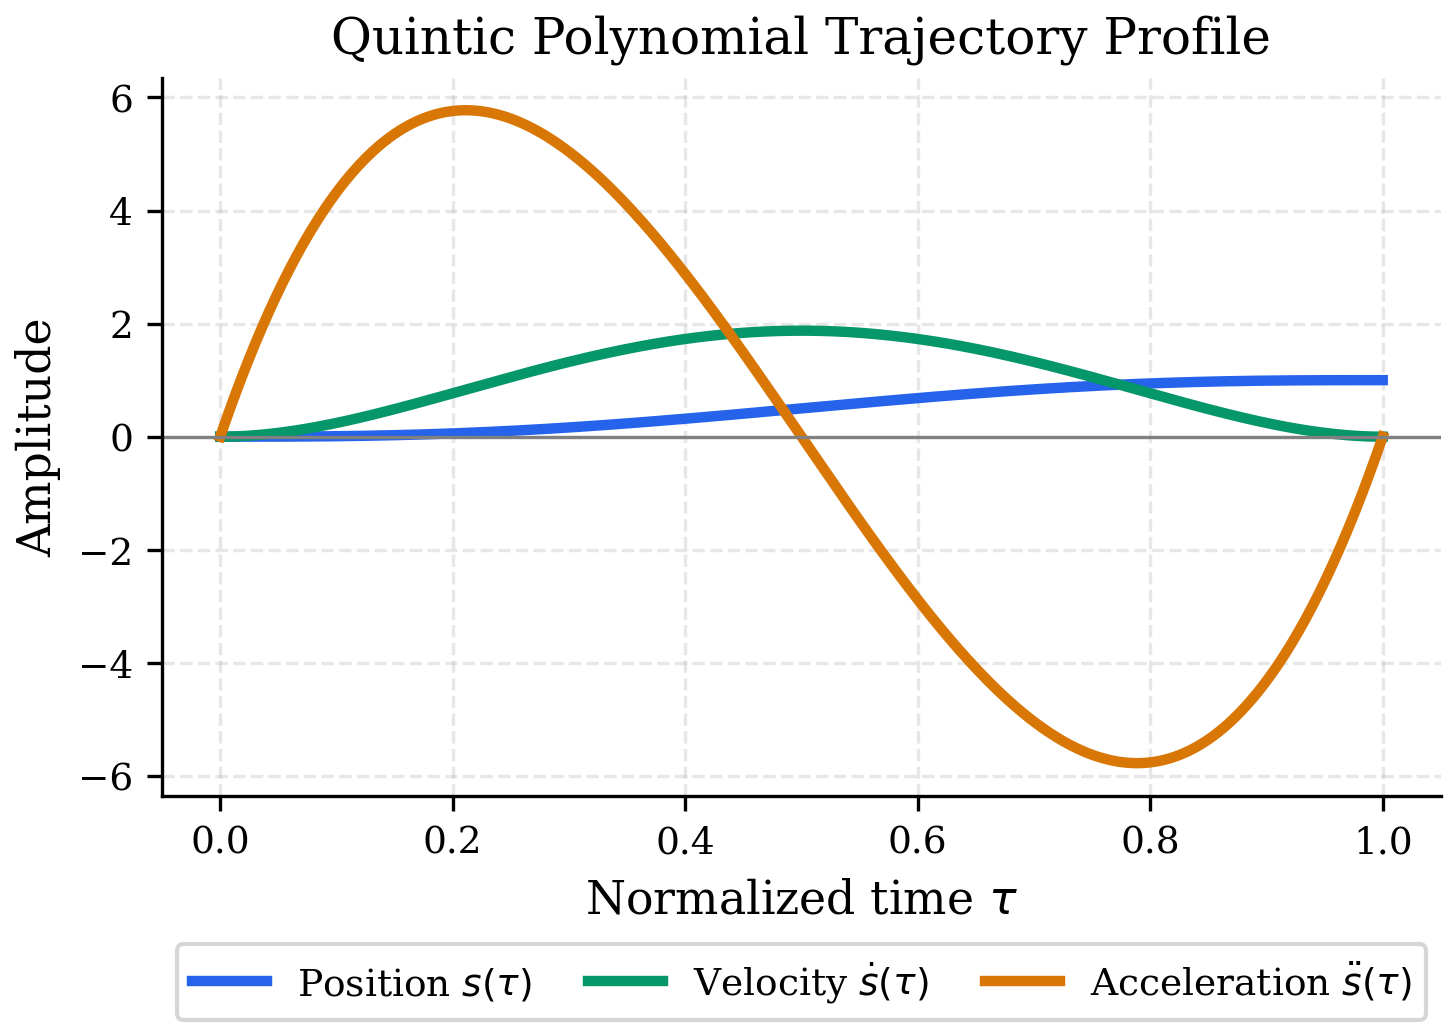
\includegraphics[width=\textwidth]{figures/quintic_pva.png}
        \caption{Quintic polynomial PVA profiles.}
        \label{fig:quintic_pva}
    \end{subfigure}
    
    \vspace{0.3cm}
    \begin{subfigure}[b]{0.85\columnwidth}
        \centering
        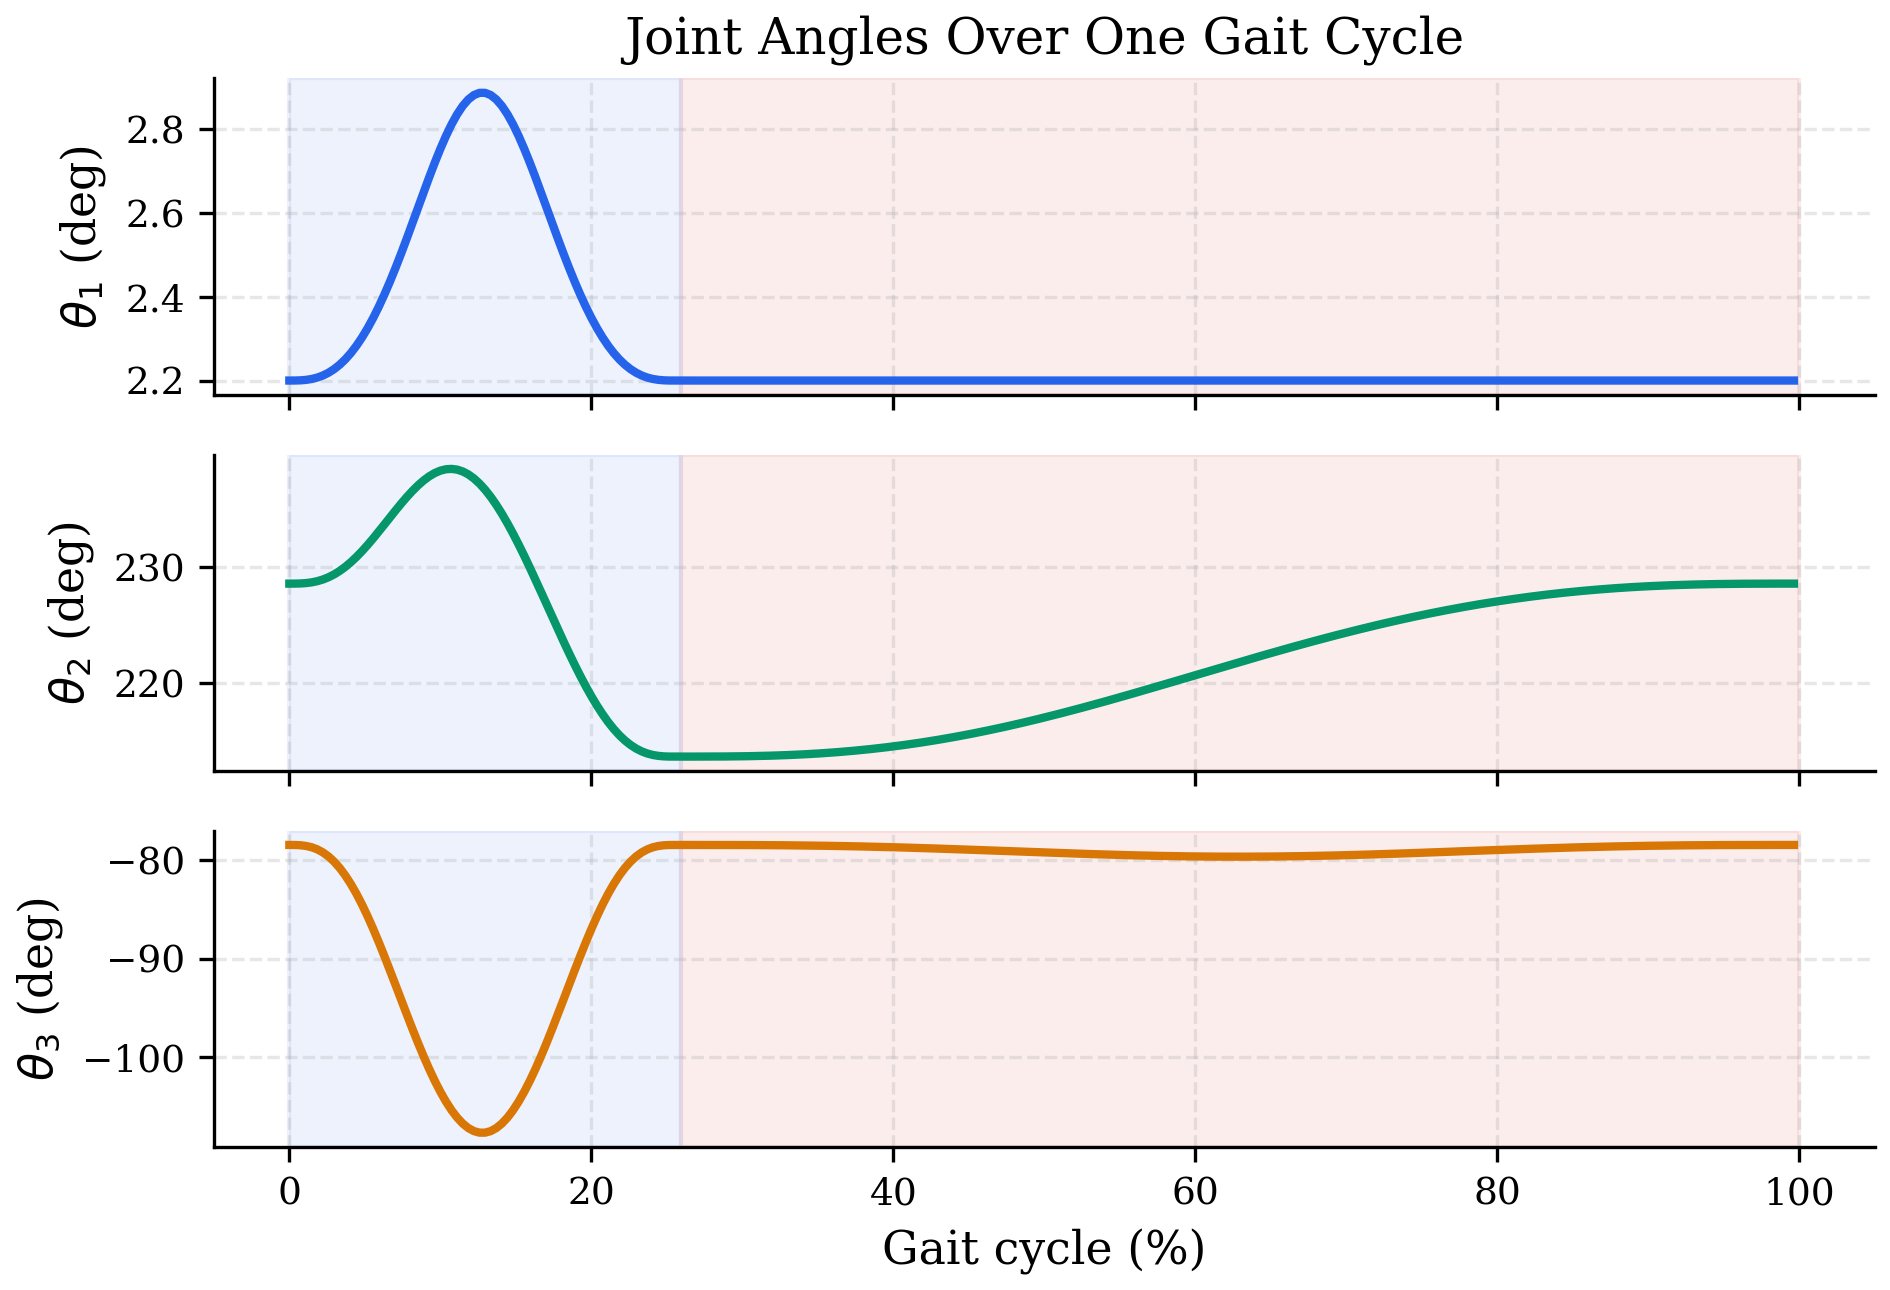
\includegraphics[width=\textwidth]{figures/joint_angles_gait.png}
        \caption{Resolved joint angles for the left front limb.}
        \label{fig:joint_angles}
    \end{subfigure}
    
    \vspace{0.3cm}
    \caption{Trajectory generation and inverse kinematic mapping.
    (a) The normalized quintic position, velocity, and acceleration
    functions dictating foot motion. (b) The resulting joint angle
    solution $\theta_i$ over one full gait cycle, with swing
    (blue, 0--26\%) and stance (red, 26--100\%) phases highlighted.}
    \label{fig:trajectory_combined}
\end{figure}
